%\chapter{Introduction générale} \label{Introduction générale}

% COVER PAGE
\centerline{\bfseries\textcolor{bleusection}{ \Huge Introduction générale}}  

\bigskip

% Figure cover
\begin{tikzpicture}
  \def\ig{%
   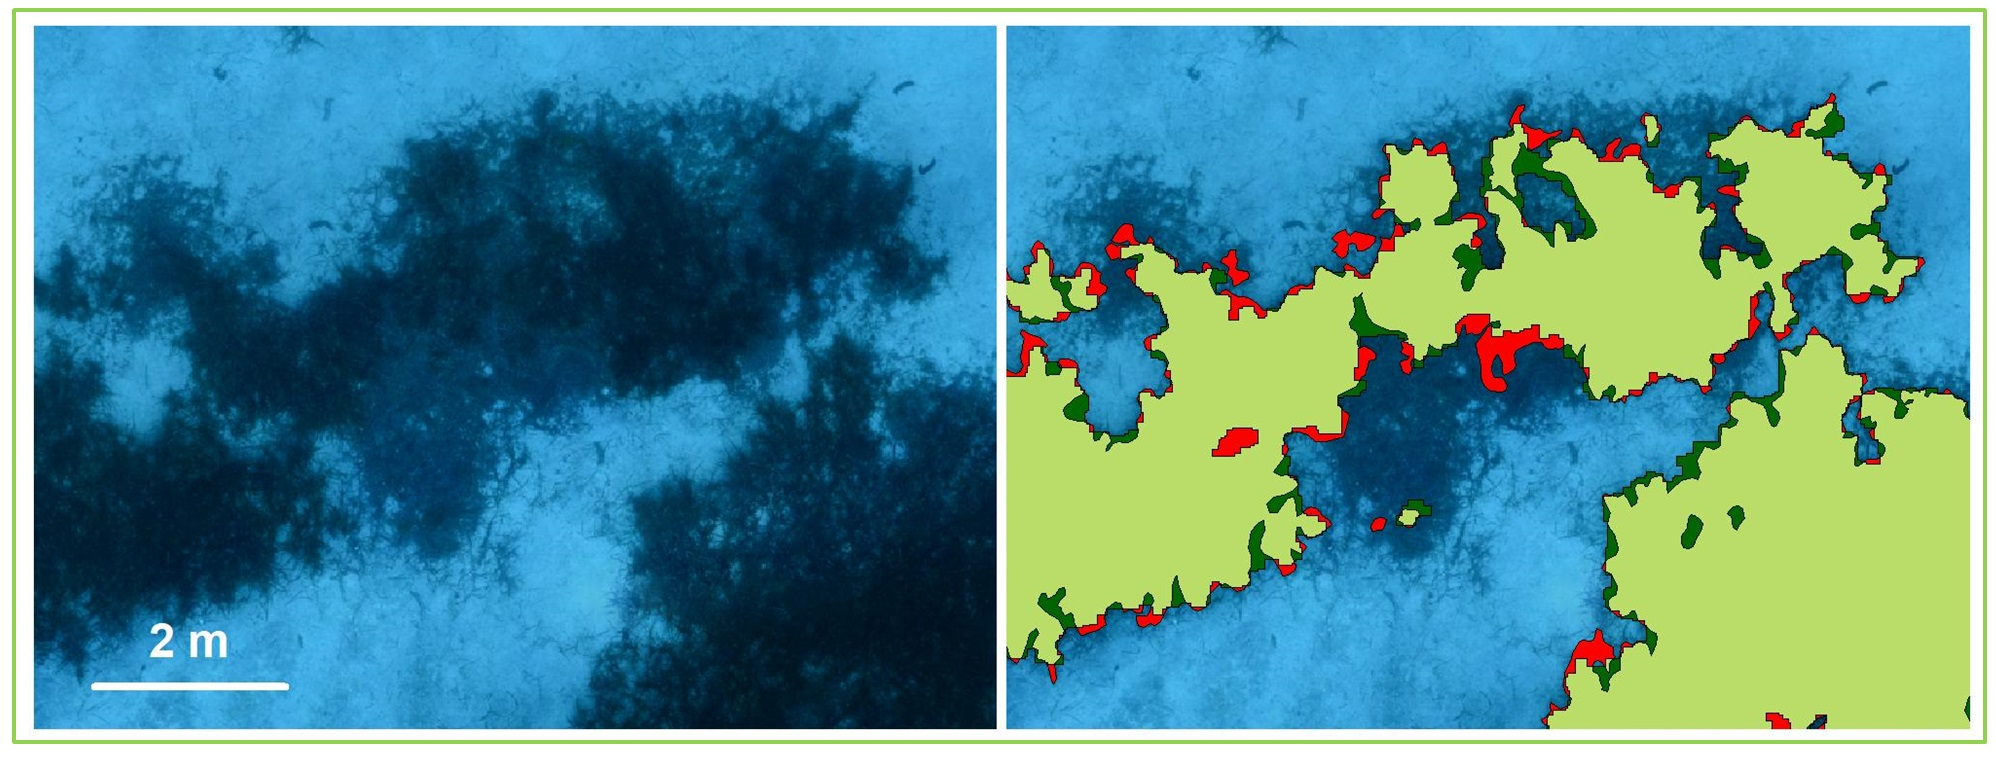
\includegraphics[width=\linewidth,keepaspectratio]{./1_intro/cover.jpg}}
 \node [inner sep=0pt](mypicture) at (0,0) {\phantom{\ig}};
 \clip[rounded corners=5mm] ($(mypicture.south west)+(\bord,\bord)$) rectangle ($(mypicture.north east)-(\bord,\bord)$);
 \node[inner sep=0pt](mypicture) at (0,0) {\ig};
\end{tikzpicture}


% Table des matières intro
{\LARGE
\begin{enumerate}[label=\textcolor{bleusection}{\arabic*}{.}, leftmargin=2cm]
  \item \nameref{intro.1}
  \item \nameref{intro.2}
  \item \nameref{intro.3}
  \item \nameref{intro.4}
\end{enumerate}
}

% DEBUT INTRO
\clearpage
\pagestyle{intro}


\section{Une biodiversité marine en danger}\label{intro.1}
\subsection{Patrons de  distribution de la biodiversité}\label{intro.1.1}

\begin{encadre}
 \label{garigue_monde}
\begin{bclogo}[couleur=encadre, couleurBord=encadre, couleurTexte=black, arrondi=0.1, marge=16,
logo=\monimage, nobreak=true]{~~\labelencadre~Le réseau de surveillance TEMPO}
 \vspace{5pt}
TEMPO est un réseau de surveillance de l’état écologique des herbiers de posidonie en Méditerranée française basé sur deux composantes importantes de l’herbier : la limite inférieure, et la profondeur intermédiaire. Ce réseau est opéré par Andromède océanologie depuis 2011 avec le soutien de l’Agence de l’eau RMC. La caractérisation de l’état écologique de l’herbier est réalisée par campagne régionale annuelle sur la période mi-mai / fin juin. Toutes régions confondues (Corse, Provence-Alpes Côte d’Azur et Occitanie) le réseau TEMPO permet l’échantillonnage de 96 sites d’herbier lors des trois années de suivi dont 53 sont localisés en limite inférieure d’herbier et 47 à la profondeur intermédiaire.
 
 \begin{figure}[H]
	\begin{center}
	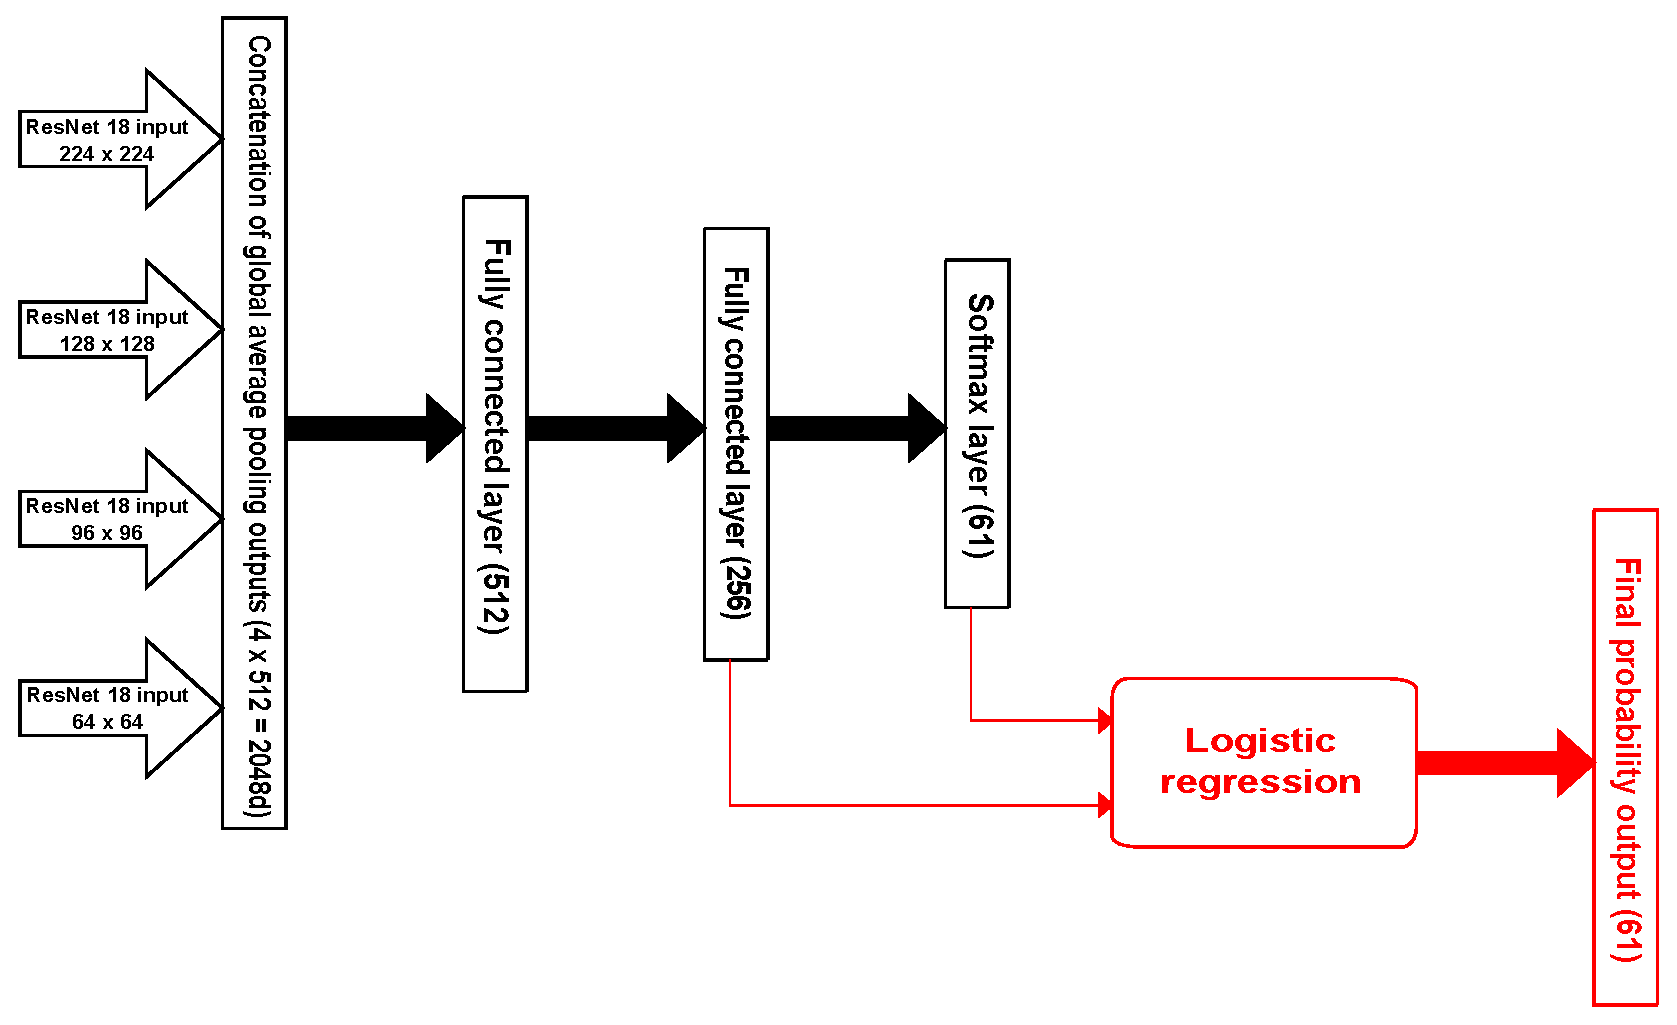
\includegraphics[width=\linewidth,keepaspectratio]{./3_chapitre1/Figure1.6}
    \end{center}
\end{figure}
 
 
\end{bclogo}
\end{encadre}

\subsection{Une biodiversité sous pression}\label{intro.1.2}
\subsection{Indicateurs de biodiversité}\label{intro.1.3}

\newpage

\section{Méthodes d'observation et de suivi des habitats marins}\label{intro.2}
\subsection{L'eau, un milieu impénétrable}\label{intro.2.1}
\subsection{Imageries sondeur et sonar: une échographie des fonds marins}\label{intro.2.2}
\subsection{Relevés plongeur: facilité d'action mais contraintes physiologiques}\label{intro.2.3}

\newpage

\section{Le contexte Méditerranéen}\label{intro.3}
\subsection{Un hotspot de biodiversité}\label{intro.3.1}
\subsection{Les herbiers de Posidonie}\label{intro.3.2}
\subsection{Les récifs coralligènes}\label{intro.3.3}

\newpage

%%% PROBLEMATIQUE %%%
\section[Problématique et objectifs scientifiques]{Problématique, questions de recherche et objectifs scientifiques}\label{intro.4}


\medskip
\noindent\textbf{\textit{Les marqueurs fonctionnels des espèces végétales présentes dans les enherbements viticoles permettent-ils d'expliquer l'impact de la communauté végétale sur les principaux services de support en viticulture ? L'étude des liens entre marqueurs fonctionnels et services de support permet-elle de sélectionner et piloter les espèces végétales pour maximiser la fourniture de services ?}}
\medskip

\noindent{Cette problématique s'est traduite en plusieurs questions de recherche :}

\begin{enumerate}[leftmargin=*]
\item \textbf{\textit{Quelles relations peut-on mettre en évidence entre les marqueurs fonctionnels des cultures de services en système viticole, et les services écosystémiques de support (protection des sols, fourniture en ressources hydriques et azotées) qu'elles rendent dans ces agrosystèmes ?}}
\item \textbf{\textit{Dans quelle mesure les marqueurs fonctionnels des communautés permettent-ils d'expliquer les services écosystémiques réalisés par les cultures de services dans ces agrosystèmes ?}}
\item \textbf{\textit{Peut-on piloter les services rendus par les cultures de services par le choix des espèces planifiées et de leurs traits, et par des interventions techniques au cours de leur cycle de croissance ?}}
\end{enumerate}

Pour y répondre, nous posons deux hypothèses de travail : $i)$ l'approche fonctionnelle par les traits des espèces et marqueurs fonctionnels des communautés est générique et peut être utilisée dans les systèmes viticoles enherbés, et $ii)$ la réalisation des services peut être évaluée par des indicateurs de fonctionnement du système sol-vigne-culture de service (stabilité structurale, couverture du sol, état hydrique et azoté du sol). 

\medskip

\noindent \textit{Les hypothèses suivantes seront testées dans cette thèse :}

\begin{description}
\item[Hypothèse 1]\label{c1:h} il existe des liens statistiques entre les marqueurs fonctionnels des communautés végétales composant les enherbements, leurs fonctions et les services qu'elles rendent aux viticulteur$\cdot$rice$\cdot$s.
\item[Hypothèse 2] : les marqueurs fonctionnels des plantes sont représentatifs du fonctionnement des espèces, et permettent de comparer les espèces et les communautés qu'elles composent en termes d'impacts sur le fonctionnement de l'agrosystème.
\item[Hypothèse 3] : les opérations techniques affectant les communautés pendant leur cycle de croissance permettent de modifier le niveau de réalisation des services 

\end{description}

En conséquence, afin de répondre à ces questions de recherche et tester les hypothèses définies, les objectifs de cette thèse sont les suivants :
\begin{enumerate}
\item la description des propriétés fonctionnelles de différentes communautés composées d'espèces planifiées et d'espèces spontanées, en particulier du point de vue de leur impact sur les ressources (eau, azote) et la structure du sol (stabilité) ;
\item l'évaluation et la description au champ des fonctions des cultures de services associées aux services de stabilisation des sols, de limitation du ruissellement, de fourniture en eau, et au service d'engrais vert ;
\item l'identification de valeurs de marqueurs fonctionnels des communautés permettant de placer le système dans une zone de compromis favorables entre services et dysservices ;
\item l'identification de leviers d'action techniques permettant le pilotage des services et dysservices par des interventions sur les cultures de services.
\end{enumerate}

La partie suivante présente la démarche générale de la thèse ainsi que les expérimentations mises en places et les mesures réalisées pour répondre aux objectifs ci-dessus.
